\documentclass[a4paper, 12pt]{article}
\usepackage[utf8]{inputenc}
\usepackage[T1]{fontenc}
\usepackage[french]{babel}
\usepackage{graphicx}
\usepackage{amsmath}
\usepackage{hyperref}
\usepackage{lmodern}
\usepackage{moreverb}
\usepackage{multicol}


\usepackage[a4paper,left=2cm,right=2cm,top=2cm,bottom=2cm]{geometry}

\pagestyle{headings}
\pagestyle{plain}


\setcounter{secnumdepth}{4}
\setcounter{tocdepth}{4}
\makeatletter


\makeatother



\makeatletter
\def\toclevel@subsubsubsection{4}
\def\toclevel@paragraph{5}
\def\toclevel@subparagraph{6}
\makeatother





\setlength{\parindent}{0cm}
\setlength{\parskip}{1ex plus 0.5ex minus 0.2ex}
\newcommand{\hsp}{\hspace{20pt}}
\newcommand{\HRule}{\rule{\linewidth}{0.5mm}}

\begin{document}

\begin{titlepage}
  \begin{sffamily}
  \begin{center}

   
    \textsc{\LARGE }\\[2cm]

    \textsc{\Large Compte rendu de Réunion}\\[1.5cm]
    \textsc{\Medium Rédigé par Ilyes ZEGHDALLOU}

    % Title
    \HRule \\[0.4cm]
    { \huge  \textsc{ StellaStone} \\
    \textsc{\Large By Novus}\\ [0.4cm] }
	

    \HRule \\[2cm]
    \textsc {Idriss BENGUEZZOU\\Mohammed ROUABAH\\Ghilas MEZIANE \\ Ilyes ZEGHDALLOU}
 \begin{figure}
     \centering
    
\includegraphics[scale=0.2]{logoUJM.png}
     \label{fig:ujm_logo}
 \end{figure}
   
    \

    \vfill

    % Bottom of the page
    {\large {} 03/10/2022}

  \end{center}
  \end{sffamily}
\end{titlepage}


\newpage
\tableofcontents

\newpage


\section{Quelle est notre ambition}
Notre entreprise Novus\footnote{Société par actions simplifiée, de création de fusée} a pour objectif de réaliser StellaStone, un logiciel permettant de simuler le voyage d'une fusée dans l'espace. \\
StellaStone, est une application de simulation destinée aussi bien à la recherche qu'à des fin pédagogiques, afin de permettre aux utilisateurs de découvrir les galaxies et les astres de notre univers.

\section{Objectifs de la réunion}
Cette réunion avait pour but de nous structurer et de nous organiser, en choisissant les outils et les moyens que nous allons utiliser durant tout le projet. 

\section{Des outils essentiels}

\subsection{Outils de rédaction}
Pour la rédaction des comptes-rendus et des différents documents, nous avons opter pour le logiciel de traitement de texte  \textbf{Word}. Nous connaissons également tous Latex, cependant nous avons conclu suite à un débat entre nous que Word nous permettrait de réaliser des documents  mieux structurés et plus attrayant visuellement. De plus, il nous sera plus aisé de rédiger sur Word de part une plus grande expérience sur ce logiciel.\\


Notre planning sera créer et tenu à jour sur \textbf{Powerpoint} et sera sous forme d'un diagramme de Gantt.
L'utilisation de Powerpoint, nous permettra de mettre au format pdf notre planning, ce que certain logiciel ou application en ligne ne nous permette pas.  \\

Il nous sera très probablement utile d'utiliser \textbf{Excel} pour la rédaction par exemple du document des tests de recette. \\

\subsection{Outils de gestion de projets}
Nous avons conclu que l'utilisation d'un logiciel de contrôle de version était incontournable. Nous avons déjà tous utilisé soit Github ou Gitlab les années précédentes. C'est pourquoi nous avons choisi de travailler sur \textbf{Gitlab} pour ce projet. \\

Certains d'entre nous utilisaient des outils de gestion de projet pour les réaliser. C'est pourquoi nous avons décidé d'utiliser \textbf{Trello}. Nous avons conclu que l'utilisation d'un logiciel de contrôle de version était incontournable. Nous avons déjà tous utilisé soit Github ou Gitlab les années précédentes. C'est pourquoi nous avons choisi de travailler sur \textbf{Gitlab} pour ce projet. \\

Certains d'entre nous utilisaient des outils de gestion de projet pour les réaliser. C'est pourquoi nous avons décidé d'utiliser \textbf{Trello}. Nous utiliserons ainsi la méthode dite de \textbf{Kanban} (méthode Agile).
\newpage

\subsection{Outils de dessin graphique}

Nous serons par la suite amené a réaliser des diagramme et des Schémas entité association. \textbf{Flowchart Maker} permet la réalisation de tels schémas en ligne et c'est ce que nous utiliserons.

\subsection{Outils de design}
Pour la réalisation de maquettes ou de design certains membre du groupe maîtrise \textbf{Figma} et \textbf{Photoshop}. C'est pourquoi nous nous efforcerons de réaliser des maquettes de qualités tout au long du semestre.\\


\section{Le planning}

 \begin{figure}[!h]
    \centering
    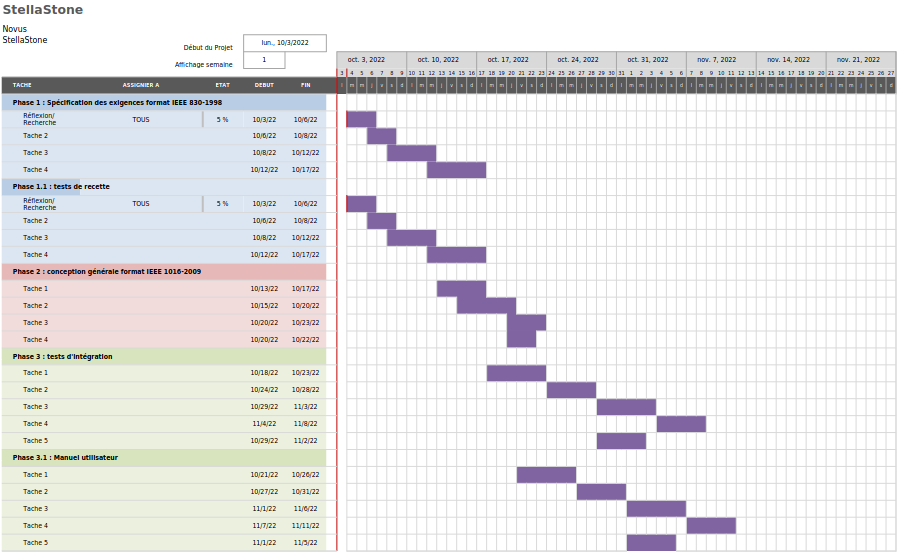
\includegraphics[scale=0.5]{Le_planning.png}
    \label{fig:Le_planning}
    \caption{Planning sous forme de diagramme de Gantt}
\end{figure}


\newpage

\begin{multicols}{2}
[
\section{Spécifications des points forts/faibles des membres du groupe }
]

\begin{itemize}
\item \textbf{BENGUEZZOU Idriss}\\
\underline{Points forts} : Rapidité et efficacité dans la recherche et la documentation - bonne organisation et structuration du travail à faire - bonne rédaction \\
\underline{Points faibles} : Orthographe -  design et style \\ 

\item \textbf{MEZIANE Ghilas}\\
\underline{Points forts} : Tenacité - Design - Orthographe et rédaction \\
\underline{Points faibles} :  Organisation  \\ \\

\item \textbf{ROUABAH Mohammed}\\
\underline{Points forts} : Imagination débordante - Patience - Altruiste et fort en communication \\
\underline{Points faibles} : Mauvaise structuration des idées \\

\item \textbf{ZEGHDALLOU Ilyes}\\
\underline{Points forts} : Tenacité - créativité - versatilité  \\
\underline{Points faibles} : Rédaction et orthographe \\
\end{itemize}
\end{multicols}

L'analyse de nos points forts et points faibles nous a permis d'anticiper nos lacunes ainsi que les problèmes auxquels nous pourrions faire face et d'établir des relations de complémentarité entre les membres du groupe afin d'optimiser le travail et le faciliter.

\section{Planification du travail de la semaine à venir:}

 \subsection{Nos débuts sur Trello} Pour optimiser la gestion de notre projet et surveiller tous ses aspects , nous allons configurer un tableau, qui listera les tâches suivant la méthode représentera \\ \\
 
\subsection{Mise en place d'un squelette Word}  Avoir une base pour nos documents est essentiel et peut nous faire gagner beaucoup de temps. C'est pour cela que nous créerons nos propres "templates" afin de pouvoir réutiliser la struture, et garder une même ossature sur tous nos documents.
\\ \\

\subsection{Création d'un repository git:} Afin de collaborer plus facilement et d'être à jour sur nos documents , nous comptons créer dès cette semaine un repository sur Gitlab. Ceci nous offrira un meilleur pilotage du projet et nous permettra d'avoir une meilleur accessibilité aux différentes versions des documents afin de rester à jour.\\ \\

\subsection{ Document de spécification des exigences: }
Réflexion et début de rédaction du document de spécification des exigences.

   
\section{Les disponibilités des membres:}
Il n'est pas aisé de trouver un créneau pour réunir tous les membres  du groupe, car chacun possède des contraintes de planning. Nous avons pu nous mettre d'accord pour se retrouver tout les Vendredi à 19h, ce qui nous permettrait de faire le point sur l'avancement réalisé durant la semaine par chaque membre du groupe, et préparer les objectifs pour la prochaine réunion. Ainsi, chaque membre pourra à son bon vouloir avancer (ou pas) ses objectifs durant le week-end.
Nous avons également prévu en cas de nécessité un second créneau, les Mardi en fin de journée, cependant aucun horaire n'a été fixé. Nous fixerons l’horaire de cette réunion exceptionnelle, uniquement si celle-ci à lieu d'être. 

\end{document}